\chapter{Hauptteil}

Sei $G$ ein planer intern 3-zusammenhängender Graph mit Aufhängungen $\{a_1,a_2,a_3\}$. Nehmen wir für einen Moment an, dass wir schon ein SLTR für $G$ gefunden haben, dann hat jeder Knoten $v$ in maximal einen inzidenten Gebiet $f$ einen flachen Winkel, den wir mit $(f,v)$ bezeichnen, und liegt auf einer Geraden. Jedes Gebiet $f$ hat genau drei Ecken, also $|f|-3$ flache Winkel. Dies liefert im Umkehrschluss eine notwendige Bedingung für die Existent einer SLTR, indem wir die Knoten den Gebieten zuordnen.

\begin{definition}[FAA]
Sei $G=(V,E,F)$ ein planer Graph, dann ist eine Flache Winkel Zuordnung, im weiteren (nach dem englischen \textit{flat-angle-assignment}) mit FAA bezeichnet, ein Matching zwischen Knoten und Gebieten, sodass:
\begin{itemize}
\item [F1] Jedem Gebiet $f$ sind genau $|f|-3$ Knoten zugeordnet.
\item [F2] Jeder Knoten $v$ ist höchstens einem Gebiet zugeordnet.
\end{itemize}
Für den Fall, dass Aufhängungen gegeben sind fordern wir zusätzlich:
\begin{itemize}
\item [F3] Die inzidenten Knoten des äusseren Gebietes, die keine Aufhängungen sind, müssen dem äusseren Gebiet zugeordnet werden.
\end{itemize}

\begin{figure}[h]
	\centering
  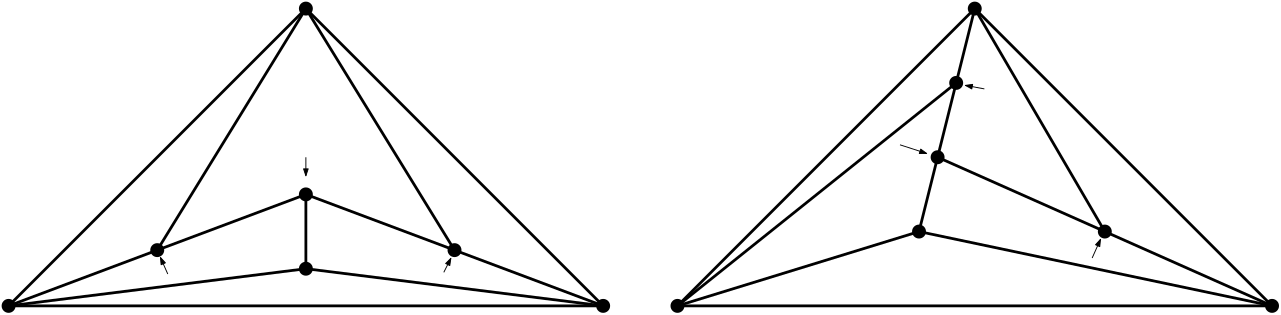
\includegraphics[width=0.9\textwidth]{faa_def.png}
  \caption{Ein planer Graph mit einer SLTR und einem FAA, dass keine SLTR induziert. Die Pfeile stellen hier die Zuweisung der Knoten zu den inneren Gebieten da.}
\end{figure}

\end{definition}

Ein planer Graph kann also nur dann eine SLTR besitzen, falls mindestens ein FAA existiert, jedoch liefert nicht jedes FAA sofort ein SLTR. Um hinreichende Konditionen für SLTRs zu erhalten werden wir uns in den nächsten beiden Abschnitten mit zwei Ansätzen nach Aerts und Felsner beschäftigen. Der erste Ansatz aus \cite{af13} liefert ein System aus harmonischen Gleichungen dessen Lösung eine SLTR liefert. In Teilen darauf basierend stellt der zweite Ansatz aus \cite{af15} einen Zusammenhang zwischen Schnyder Woods und FAAs her und die Existenz passender Paare impliziert wieder die Existenz von SLTRs.

\section{Harmonische Funktionen}

Wir werden die Beweise zu den in diesem Abschnitt aufgestellten Präpositionen und Theoremen übergehen. Der interessierte Leser sei, sofern nicht anders angegeben auf \cite{af13} verwiesen. Zum Einstieg formulieren wir eine weitere Definition um dann eine Beobachtung zu SLTRs festzuhalten.

\begin{definition}[Begrenzende Zykel und kombinatorisch konvexe Ecken]
Sei $G$ ein planer Graph mit Aufhängungen $\{a_1,a_2,a_3\}$ und einem FAA $\phi$ von G. Sei $H$ ein zusammenhängender Teilgraph von G und $\gamma=\gamma(H)$ der H umrandende Weg in G, also die Kanten und Knoten des äusseren Gebiets von H, wobei hier Knoten und Kanten mehrfach vorkommen können. Wir werden so erhaltene $\gamma$ als \textit{begrenzende Zykel} bezeichnen. $int(\gamma)$ sei die Menge aller Knoten, Kanten und Gebiete aus G die im inneren von $\gamma$ oder auf $\gamma$ liegen. Einen Knoten $v$ aus $\gamma$ bezeichnen wir als \textit{kombinatorisch konvexe Ecke} von $\gamma$ im Bezug auf $\phi$, falls gilt:
\begin{itemize}
\item [E1] $v$ ist eine Aufhängung, oder
\item [E2] $v$ ist nicht durch $\phi$ zugeordnet und es existiert eine Kante $e = (v,w)$ mit $e \notin int(\gamma)$, oder
\item [E3] $v$ ist einem Gebiet $f$ zugeordnet, $f \notin int(\gamma)$ und es existiert eine Kante $e = (v,w)$, sodass $e \notin int(\gamma)$.
\end{itemize}

\end{definition}

\begin{figure}[h]
	\centering
  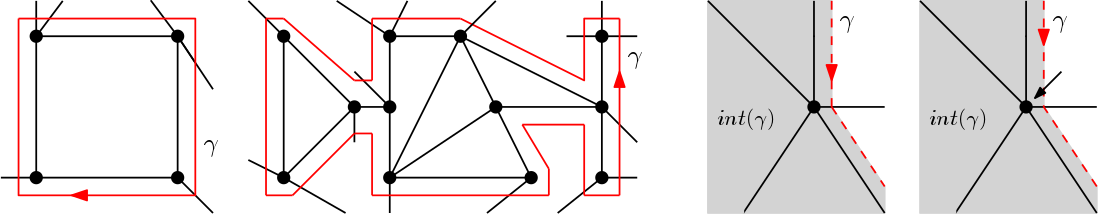
\includegraphics[width=0.9\textwidth]{corner_def.png}
  \caption{Auf der linken Seite zwei Beispiele für \textit{begrenzende Zykel} und rechts für \textit{kombinatorisch konvexe Ecken} mit und ohne zugewiesenem Knoten.}
\end{figure}

Es lässt sich für SLTRs leicht zeigen, dass für jeden begrenzenden Zykel $\gamma$, der nicht von einem Pfad induziert wird, gilt, dass er mindestens drei kombinatorisch konvexe Ecken besitzt. Die folgende Präposition nach \cite[Prop 2.2, Prop 2.4]{af13} verallgemeinert diese Beobachtung.

\begin{proposition}\label{com_prop}
Sei $G$ ein planer Graph der eine SLTR $\Gamma$ zulässt. Sei weiter $\phi$ das von $\Gamma$ induzierte FAA und $H$ ein zusammenhängender Teilgraph von G. Falls $v$ eine geometrisch konvexe Ecke in $\Gamma$ ist, dann ist $v$ auch eine kombinatorisch konvexe Ecke hinsichtlich $\phi$. Somit gilt:
\begin{itemize}
\item [E4] Jeder begrenzende Zykel $\gamma$, der nicht von einem Pfad induziert wird, hat hinsichtlich $\phi$ mindestens drei kombinatorisch konvexe Ecken.
\end{itemize}

\end{proposition}

Proposition \ref{com_prop} liefert also eine notwendige Bedingung damit ein FAA von einer SLTR induziert sein kann. Dies ist sogar eine hinreichende Bedingung wie im Verlauf des Abschnittes in Theorem \ref{com_theo} gezeigt werden wird. Wir nennen ein FAA das [E4] erfüllt im Weiteren \textit{Gutes-FAA} oder kurz \textit{GFAA}. Aerts und Felsner zeigen, dass ein Gutes-FAA eine \textit{Kontaktfamilie von Pseudosegmenten} induziert die \textit{dehnbar} ist und sich somit geradlinig darstellen lässt.

\begin{definition}[Kontaktfamilie von Pseudosegmenten]

Eine \textit{Kontaktfamilie von Pseudosegmenten} ist eine Familie $\Sigma = \{c_i\}_i$ von einfachen Kurven $$c_i:[0,1] \to \mathbb{R}^2, \text{ mit } c_i(0) \neq c_i(1),$$ sodass alle Kurven $c_i,c_j$ mit $i \neq j$ maximal einen gemeinsamen Punkt haben. Dieser Punkt muss dann ein Endpunkt von mindestens einer der Kurven sein.

\end{definition}

Ein GFAA $\phi$ liefert eine Relation $\rho$ auf den Kanten von G. Zwei Kanten $(v,w),(v,u)$, beide adjazent zu $f$, stehen genau dann in Relation, falls $\phi(v)=f$, wenn also $(v,w)$ und $(v,u)$ auf der selben Seite von $f$ in der SLTR liegen. Der transitive Abschluss dieser Relation liefert eine Äquivalenzrelation $\rho$. Die Aquivalenzklassen von $\rho$ bilden eine Kontaktfamilie von Pseudosegmenten. Nennen wir die Äquivalenzklassen von $\rho$ Kurven, dann liefert [F2], dass jeder Knoten nur im inneren von einer Kurve liegt und sich die Kurven nicht kreuzen. Weiter hat jede Kurve unterschiedliche Anfangs- und Endpunkte und kann sich nicht selbst berühren, da der resultierende begrenzende Zykel $\gamma$ nur eine beziehungsweise zwei kombinatorisch konvexe Ecken, was ein Widerspruch zu [E4] wäre. Analog können zwei Kurven nicht ihre Anfangs- und Endpunkte teilen.\
Für eine von einem FAA $\phi$ induzierte Kontaktfamilie schreiben wir auch $\Sigma_{\phi}$.

\begin{figure}[h]
	\centering
  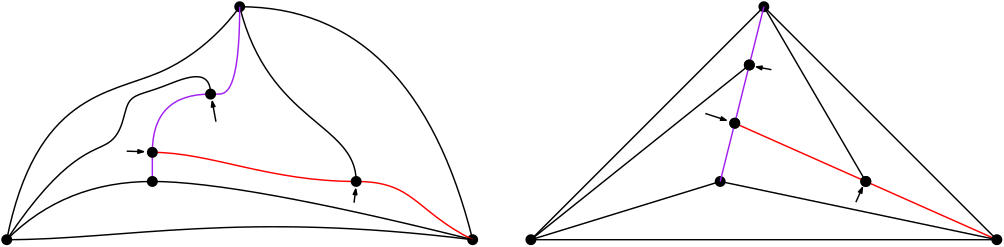
\includegraphics[width=0.9\textwidth]{pseudo_seg.png}
  \caption{Die Kanten von G als Kontaktfamilie von Pseudosegmenten induziert durch die Äquivalenzrelation. In rot und grün die beiden Äquivalenzklassen bzw. Kurven, die mehr als eine Kante beinhalten.}
\end{figure}

\begin{definition}
Sei $\Sigma$ ein Kontaktfamilie von Pseudosegmenten und $S\subseteq\Sigma$. Wir nennen einen Punkt $p\in S$ einen \textit{freien Punkt}, falls
\begin{itemize}
\item p ist ein Endpunkt eines Pseudosegmentes aus S.
\item p liegt nicht im Inneren eines Pseudosegmentes aus S.
\item p liegt am äusseren Rand von S.
\item p ist entweder eine Aufhängung von G, oder berührt ein Pseudosegment, welchen nicht zu S gehört.
\end{itemize} 
\end{definition}

\begin{lemma}\cite[Lemma 2.8]{af13}
Sei $\phi$ ein Gutes-FAA auf einem planen und intern 3-zusammenhängenden Graphen. Dann hat gilt: 
\begin{itemize}
\item [E5] jede Teilmenge $S \subseteq \Sigma_{\phi}$ mit $|S| \geq 2$ hat mindestens 3 freie Punkte.
\end{itemize}
\end{lemma}

Betrachten wir also einen planen, intern 3-zusammenhängenden Graphen $G$ mit Aufhängungen $\{a_1,a_2,a_3\}$ und einem GFAA $\phi$. Wenn wir die von $\phi$ induzierte Kontaktfamilie $\Sigma_{\phi}$ mit geradlinigen Segmenten darstellen können, dann haben wir eine zu $\phi$ passende SLTR für G gefunden. Für den Fall, dass eine solche Darstellung existiert, können wir für die resultierenden Koordinaten der Segmente und somit auch der Knoten von G Gleichungen aufstellen, die diese erfüllen müssten.

\begin{definition}[Harmonische Funktionen]

\end{definition}

Nehmen wir für den Moment an, dass wir eine Darstellung gefunden haben, dann gilt für jeden inneren Knoten $v$ auf einem Segment, dass er auf einer Gerade zwischen seinen beiden benachbarten Knoten $u,w$ auf dem Segment liegen muss. Diese Eigenschaft liefert 

\section{Ecken kompatible Paare}
